\subsection{Seismic attributes}
\label{subsec:seismic-attributes}

Seismic attributes are quantitative measures derived from seismic data, which describe various aspects of the subsurface geology.
Over the past few decades, seismic attributes have become an indispensable tool in the exploration and production of hydrocarbons, mineral resources, and the management of geohazards.
They have significantly contributed to the understanding of complex geological settings and have improved the accuracy of reservoir characterization and prediction.

Seismic data, which is obtained through the use of controlled seismic sources and an array of receivers, is used to create images of the subsurface geology.
The acquired data is processed and interpreted to reveal geological features, such as faults, fractures, and rock properties.
However, seismic data can be challenging to interpret due to the complex nature of the subsurface geology and the limitations of seismic imaging techniques.

The evolution of seismic attributes is explored by Barnes and Arthur~\cite{barnes2001seismic}, Chopra \etal~\cite{chopra2005seismic}, Fawad \etal~\cite{fawad2020seismic}, and Taner and Turhan~\cite{taner2001seismic}.
This concept was first introduced in the late 1970s as a means to enhance the interpretation of seismic data.
Since then, the field has experienced significant advancements, driven by the growth in computational power and the development of innovative seismic processing and interpretation techniques.
Seismic attributes can be broadly classified into five categories:

\begin{itemize}
    \item \textbf{Amplitude-based attributes}: These attributes are derived from the amplitude of the seismic waveforms and are used to analyze variations in rock properties, fluid content, and stratigraphy.
        Common examples of amplitude-based attributes include average amplitude, root-mean-square amplitude, and instantaneous amplitude;
    \item \textbf{Frequency-based attributes:} These attributes focus on the frequency content of the seismic data and can reveal information about the thickness and composition of subsurface layers.
        Examples of frequency-based attributes include spectral decomposition, dominant frequency, and instantaneous frequency;
    \item \textbf{Time and spatial-based attributes:} These attributes describe the geometrical and temporal properties of seismic events, such as the continuity, dip, and azimuth of reflectors.
        Some examples of time and spatial-based attributes are coherence, curvature, and semblance;
    \item \textbf{Mitigation attributes:} These attributes are designed to reduce the impact of noise and other artifacts in the seismic data, improving the overall quality and interpretability of the data.
        Examples of mitigation attributes include random noise attenuation, multiple suppression, and ground roll removal;
    \item \textbf{Texture attributes:} These attributes characterize the texture or patterns within the seismic data, providing insights into geological features such as fractures, channels, and stratigraphic boundaries.
        Texture attributes can be computed using techniques such as gray-level co-occurrence matrices, wavelet decomposition, and local binary patterns.
\end{itemize}

To illustrate how seismic attributes are used, Figure~\ref{fig:seismic-complex-attr} shows a sample of two complex seismic attributes derived from the amplitude of a sample seismic data.
The envelope of the amplitude, which is ilustrated by Figure~\ref{fig:seismic-envelope}, highlights the presence of a possible hydrocarbons reservoir.
Figure~\ref{fig:seismic-inst-phase} shows the instantaneous phase of the seismic data, which defines the phase of the seismic wavelet at each sample.

\begin{figure}[htb!]
    \captionsetup[subfigure]{justification=centering}
    \centering

    \subfloat[][Amplitude (raw data)]{
        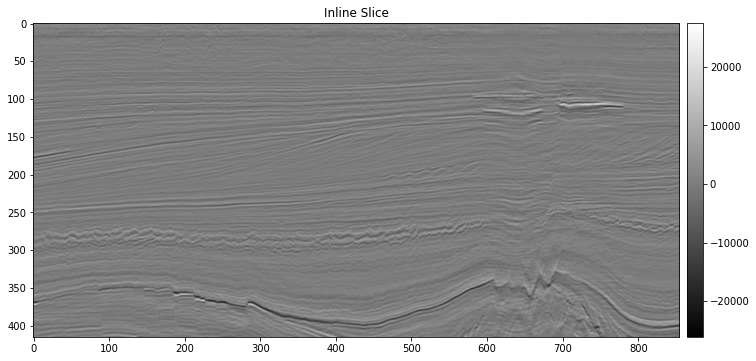
\includegraphics[height=4cm]{images/seismic-amplitude.png}
        \label{fig:seismic-raw-data}
    }
    
    \subfloat[][Amplitude envelope (the red arrow highlights a possible hydrocarbons reservoir)]{
        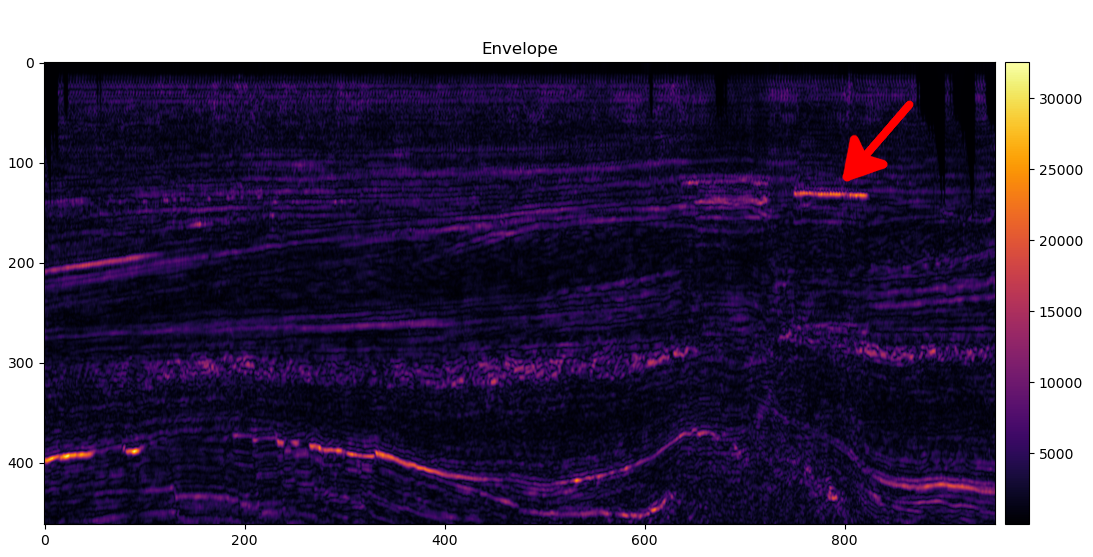
\includegraphics[height=4cm]{images/seismic-envelope.png}
        \label{fig:seismic-envelope}
    }
    \subfloat[][Instantaneous phase]{
        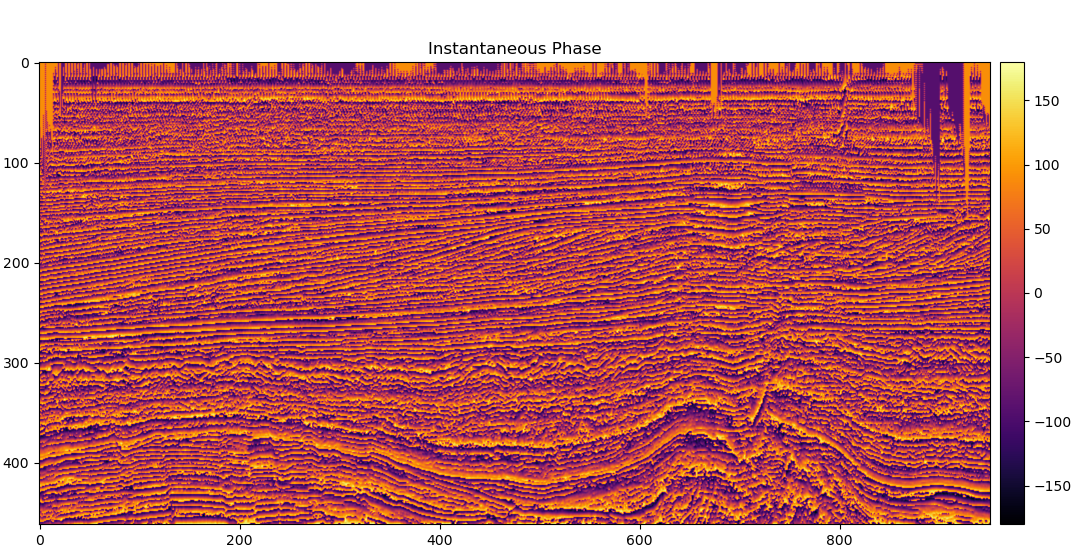
\includegraphics[height=4cm]{images/seismic-inst-phase.png}
        \label{fig:seismic-inst-phase}
    }

    \caption{Sample of two complex seismic attributes derived from the amplitude to the inline}
    \label{fig:seismic-complex-attr}
\end{figure}

As explained in the previous example, the integration of seismic attributes into the interpretation workflow allows geoscientists to extract valuable information from seismic data more efficiently.
Seismic attributes can be combined with other data, such as well logs and geological models, to provide a comprehensive understanding of the subsurface geology.
Furthermore, advanced machine learning and data analytics techniques have enabled the development of multi-attribute analysis, which involves the simultaneous examination of multiple attributes to identify patterns and relationships that may not be apparent when considering individual attributes.

Seismic attributes play a crucial role in the analysis and interpretation of seismic data by providing quantitative measures of subsurface geology.
They enhance the understanding of complex geological settings, improve reservoir characterization, and aid in the prediction of subsurface resources.
As the field continues to evolve, the integration of seismic attributes with other data sources and advanced computational techniques will further advance the state of knowledge in the field and enable more accurate and efficient exploration and production efforts.
